\documentclass[aspectratio=169,notes]{beamer}
% \documentclass[aspectratio=169]{beamer}
\usetheme[faculty=phil]{fibeamer}
\usepackage{polyglossia}
\setmainlanguage{english} %% main locale instead of `english`, you
%% can typeset the presentation in either Czech or Slovak,
%% respectively.
\setotherlanguages{russian} %% The additional keys allow
%%
%%   \begin{otherlanguage}{czech}   ... \end{otherlanguage}
%%   \begin{otherlanguage}{slovak}  ... \end{otherlanguage}
%%
%% These macros specify information about the presentation
\title[AGLA1]{Analytical Geometry and Linear Algebra I, Lab 4} %% that will be typeset on the
\subtitle{Matrix Rank \\ Test 1 Solutions \\ Q/A session   
         } %% title page.
\author{Oleg Bulichev}
%% These additional packages are used within the document:
\usepackage{ragged2e}  % `\justifying` text
\usepackage{booktabs}  % Tables
\usepackage{tabularx}
\usepackage{tikz}      % Diagrams
\usetikzlibrary{calc, shapes, backgrounds}
\usepackage{amsmath, amssymb}
\usepackage{url}       % `\url`s
\usepackage{listings}  % Code listings
% \usepackage{subfigure}
\usepackage{floatrow}
\usepackage{subcaption}
\usepackage{mathtools}
\usepackage{todonotes}
\usepackage{fontspec}
\usepackage{multicol}
\usepackage{pdfpages}
\usepackage{wrapfig}
\usepackage{animate}
\usepackage{booktabs}
\usepackage{multirow}

\graphicspath{{resources/}}
\frenchspacing

\setbeamertemplate{caption}[numbered]
\usetikzlibrary{graphs}

% \usepackage[backend=biber,style=ieee,autocite=footnote]{biblatex}
% \addbibresource{biblio.bib}
% \DefineBibliographyStrings{english}{%
%   bibliography = {References},}

\newcommand{\oleg}[2][] {\todo[color=red, #1] {OLEG:\\ #2}}
\newcommand{\fbckg}[1]{\usebackgroundtemplate{\includegraphics[width=\paperwidth]{#1}}}%frame background

\usepackage[framemethod=TikZ]{mdframed}
\newcommand{\dbox}[1]{
\begin{mdframed}[roundcorner=3pt, backgroundcolor=yellow, linewidth=0]
\vspace{1mm}
{#1}
\vspace{1mm}
\end{mdframed}
}

\begin{document}
\setlength{\abovedisplayskip}{0pt}
\setlength{\belowdisplayskip}{0pt}
\setlength{\abovedisplayshortskip}{0pt}
\setlength{\belowdisplayshortskip}{0pt}

\fbckg{fibeamer/figs/title_page.png}
\frame[c]{\setcounter{framenumber}{0}
    \usebeamerfont{title}%
    \usebeamercolor[fg]{title}%
    \begin{minipage}[b][6.5\baselineskip][b]{\textwidth}%
        \textcolor{black}{\raggedright\inserttitle}
    \end{minipage}
    % \vskip-1.5\baselineskip

    \usebeamerfont{subtitle}%
    \usebeamercolor[fg]{framesubtitle}%
    \begin{minipage}[b][3\baselineskip][b]{\textwidth}
        \raggedright%
        \insertsubtitle%
    \end{minipage}
    \vskip.25\baselineskip
}
%   \frame[c]{\maketitle}
\note{
    \begin{enumerate}
        \item Чилл пара

    \end{enumerate}
}

\fbckg{fibeamer/figs/common.png}


\begin{frame}[c]{Questions from the class}
\framesubtitle{}
\centering
    \textit{ \Large No questions for today}
\end{frame}

\begin{frame}[t]{Matrix Rank}
    \framesubtitle{Definition}
        \textbf{$N_r(A)$} --- max number of \textbf{lineary independent} rows of matrix $A$.
    
        \textbf{$N_c(A)$} --- max number of \textbf{lineary independent} columns of matrix $A$.
    
        \begin{equation*}
            Rank(A) = N_r(A) = N_c(A)
        \end{equation*}
    \bigskip
    
        \centering
        The rank of the matrix is how many of the rows (columns) are <<unique>>: not formed out by other rows (columns).
    \end{frame}
    
    \begin{frame}[t]{Matrix Rank}
    \framesubtitle{Motivation}
        \begin{itemize}
            \item Computation of the number of solutions of a system of linear equations.
            \item Analysis of the linear dependency of rows and columns.
            \item Applications in Control Theory (next year): observability and controllability.
        \end{itemize}
    \end{frame}
    
    \begin{frame}[t]{Matrix Rank}
    \framesubtitle{How to find}
        There are 3 ways:
        \begin{enumerate}
            \item \textbf{Look at matrix} and find linear dependencies.
            \item \textbf{Reduced form} (transform matrix to upper triangular form (The first part of the algorithm for finding inverse matrix).
            \item \textbf{Minor method} (\href{http://www.mathprofi.ru/rang_matricy.html}{Метод окаймляющих миноров} ) \textit{not popular in western education}.
        \end{enumerate}
    \end{frame}


\begin{frame}[t]{Matrix Rank}
\framesubtitle{Case Study (on whiteboard)}
Calculate the rank of the following matrix: $\begin{bmatrix}1&2&3\\2&3&4\\1&1&1\end{bmatrix}$. \medskip

\alert{\Large Answer: 2}
\end{frame}

\begin{frame}[t]{Matrix Rank}
\framesubtitle{Task 2}
Determine the ranks of the following matrices for all real values of parameter $\alpha$:
\begin{enumerate}

    \item $\begin{bmatrix}1&\alpha&-1&2\\2&-1&\alpha&5\\1&10&-6&1\end{bmatrix}$;
    \item $\begin{bmatrix}1&1&1\\1&\alpha&\alpha^2\\1&\alpha^2&\alpha\end{bmatrix}$;
\end{enumerate}
\end{frame}

\begin{frame}[t]{How to get out of an exam}
    \framesubtitle{Video}
    \vspace{-0.6cm}
    \begin{figure}[H]
        \href{https://youtu.be/eiLF4zRA634}{
            \centering
\includegraphics[height=6cm,width=1\textwidth,keepaspectratio]{meme.jpg}}
        % \caption{Click on a picture for a video}
        \label{fig:meme.jpg}
    \end{figure}
\end{frame}

\begin{frame}[t]{Test 1, Solutions}
\framesubtitle{Task 1}
(2 points) For each of the following statements mark it as True or False. Justify each answer.
\smallskip
% \vskip


\begin{enumerate}

\begin{tabular}[b]{p{10cm}|p{2cm}}

\hline
   \item  If matrix $B$ is produced by interchanging two columns of matrix $A$, then $\det (B) = -\det (A) $. 
   
   Explain your answer in $2\times 2$ case. &    \\ 
%   \hline
%     \item The result of Scalar triple product operation is a vector. & \\
    \hline
    \item For any square matrix $A$ there exists exactly one inverse matrix. & \\
    \hline
    \end{tabular}
\end{enumerate}
\end{frame}

\begin{frame}[t]{Test 1, Solutions}
\framesubtitle{Task 2}
(2 points) Decompose the vector $\textbf{p} = (1, 2, 3)$ into components parallel and perpendicular to the vector $\textbf{q} = (1, -2, 2)$.
\end{frame}

\begin{frame}[t]{Projection}
    \framesubtitle{Definition}
    \vspace{-0.3cm}
    \begin{columns}[T,onlytextwidth]
        \begin{column}{0.5\textwidth}
            The \textit{vector projection} of a vector $\mathbf {a}$ on (or onto) a nonzero vector $\mathbf {b}$, sometimes denoted $\operatorname {proj} _{\mathbf {b} }\mathbf {a}$  is the orthogonal projection of $\mathbf {a}$ onto a straight line parallel to $\mathbf {b}$.
        \end{column}
        \begin{column}{0.49\textwidth}
            \vspace{-1cm}
            \begin{figure}[H]
                \centering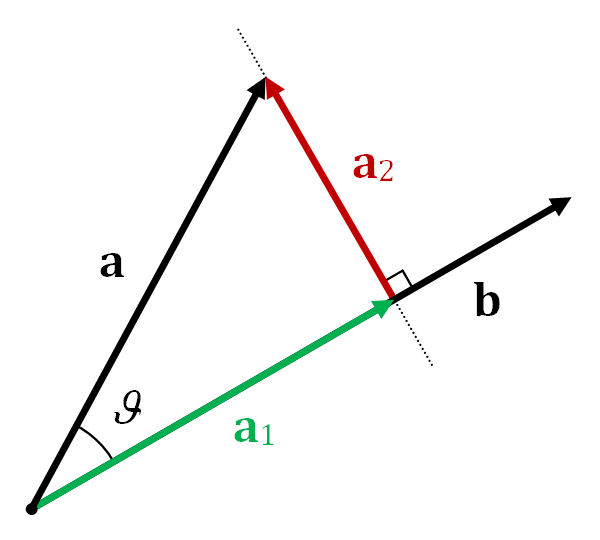
\includegraphics[height=3cm,width=1\textwidth,keepaspectratio]{Projection_and_rejection.png}
                \caption*{Projection of $\mathbf{a}$ on $\mathbf{b}$ ($\mathbf{a}_1$), and rejection of $\mathbf{a}$ from $\mathbf{b}$ ($\mathbf{a}_2$)}
                \label{fig:Projection_and_rejection.png}
            \end{figure}
        \end{column}
    \end{columns}
    \textbf{Where it can be used:}
    \vspace{-0.5cm}
    \begin{multicols}{2}
        \begin{itemize}
            \item Maps
            \item Blueprints
            \item Fitting algorithms (Least squares)
            \item Reduce matrix dimension
            \item Reinforcement Learning (RL) fitness functions
        \end{itemize}
    \end{multicols}
\end{frame}

\begin{frame}[t]{Projection (1)}
    \framesubtitle{}
    \begin{figure}[H]
        \centering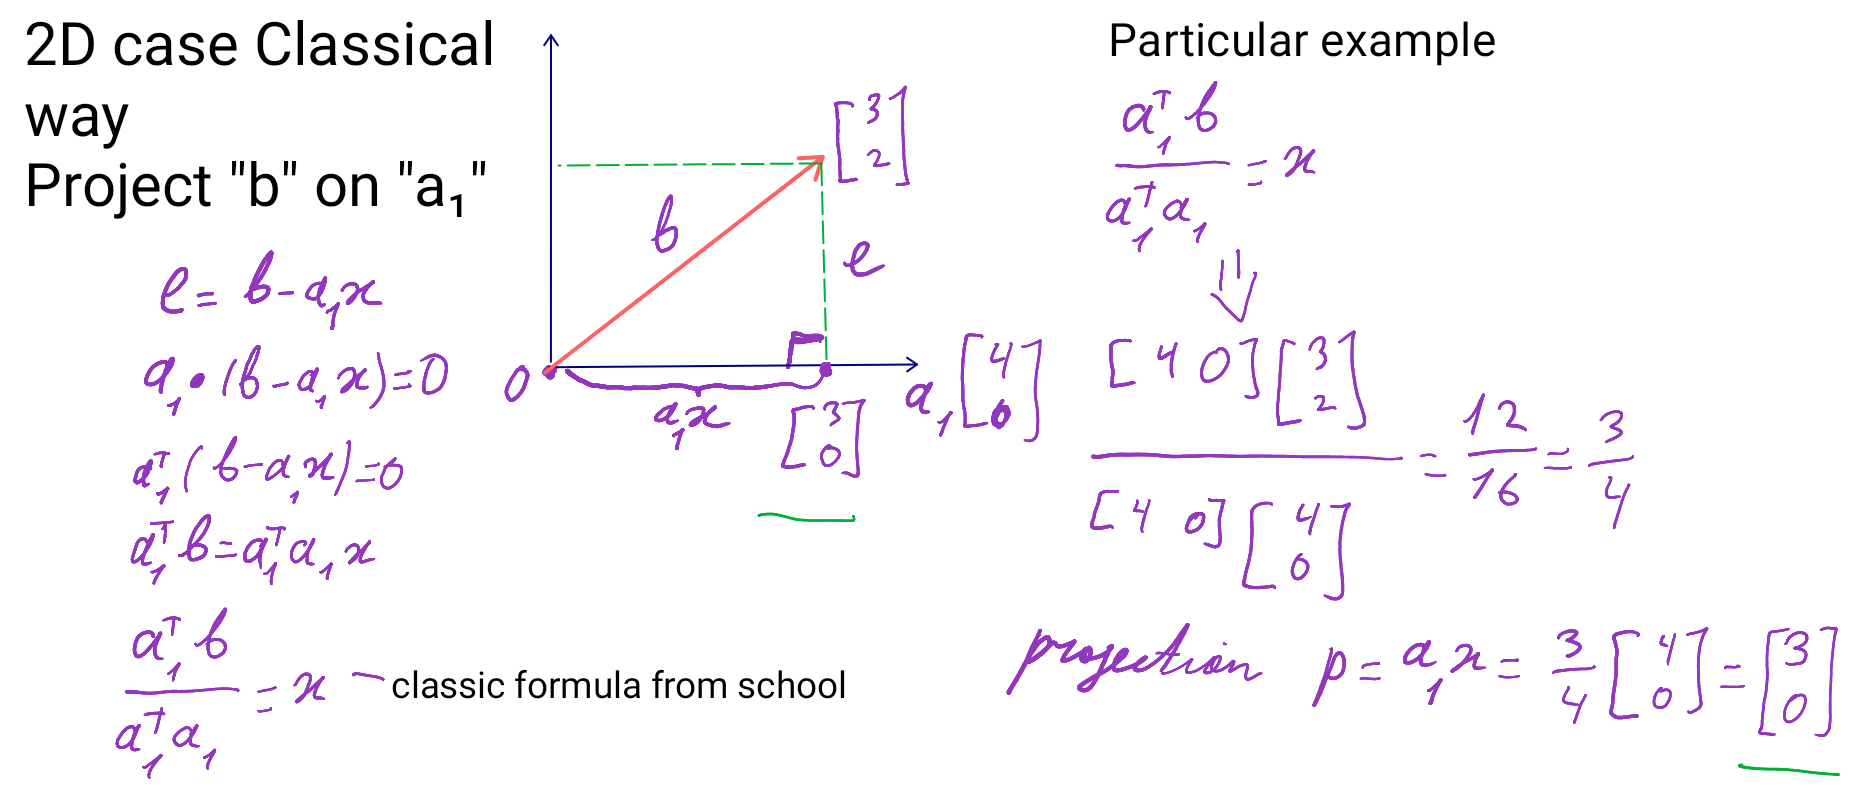
\includegraphics[height=6cm,width=1\textwidth,keepaspectratio]{AGLA2_for_slides_1.png}
        % \caption{caption_name}
        \label{fig:AGLA2_for_slides_1.png}
    \end{figure}
\end{frame}

\begin{frame}[t]{Projection (2)}
    \framesubtitle{}
    \begin{figure}[H]
        \centering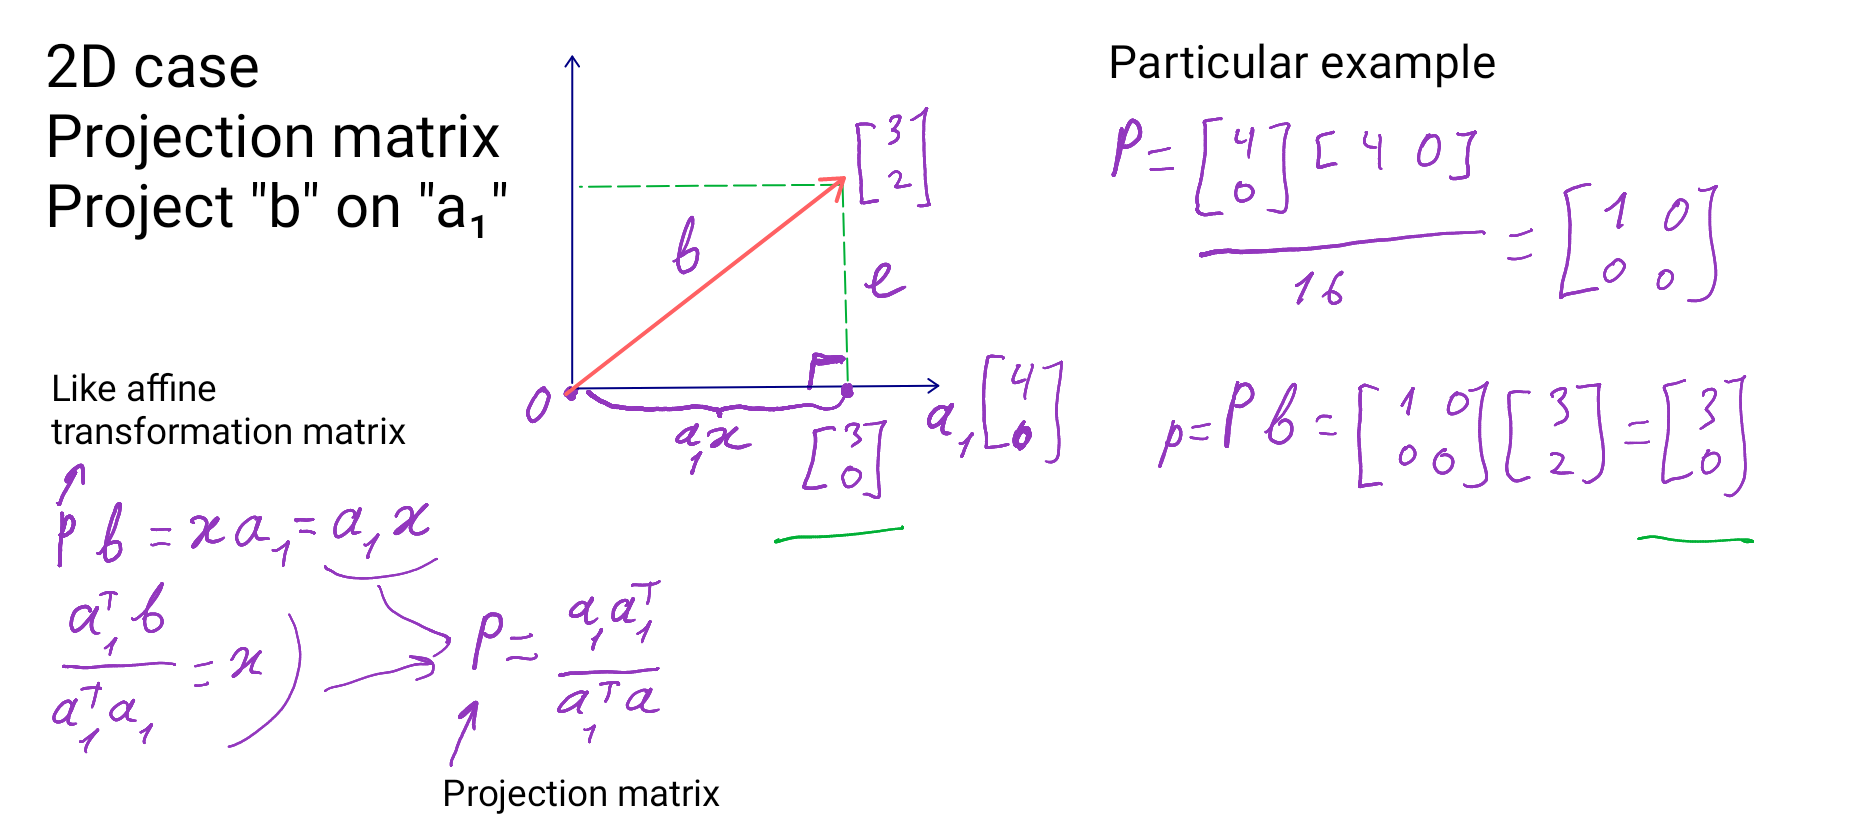
\includegraphics[height=6cm,width=1\textwidth,keepaspectratio]{AGLA2_for_slides_2.png}
        % \caption{caption_name}
        \label{fig:AGLA2_for_slides_2.png}
    \end{figure}
\end{frame}

\begin{frame}[t]{Projection (3)}
    \framesubtitle{}
    \begin{figure}[H]
        \centering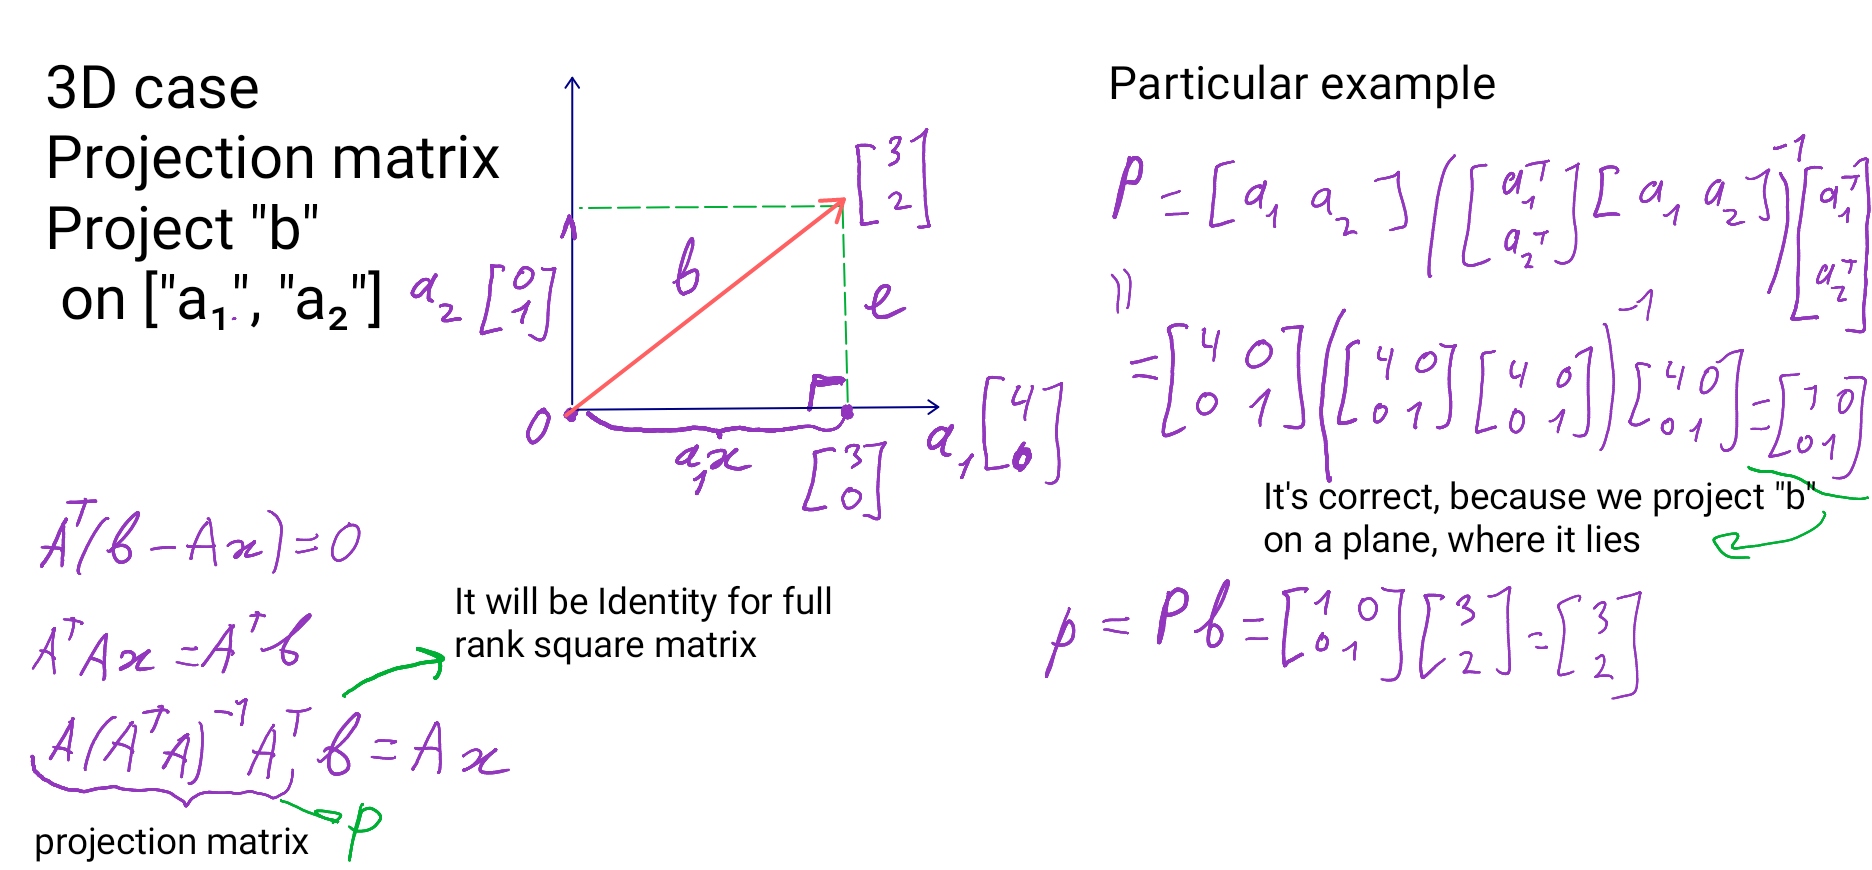
\includegraphics[height=6cm,width=1\textwidth,keepaspectratio]{AGLA2_for_slides_3.png}
        % \caption{caption_name}
        \label{fig:AGLA2_for_slides_3.png}
    \end{figure}
\end{frame}

\begin{frame}[t]{Projection (4)}
    \framesubtitle{}
    \begin{figure}[H]
        \centering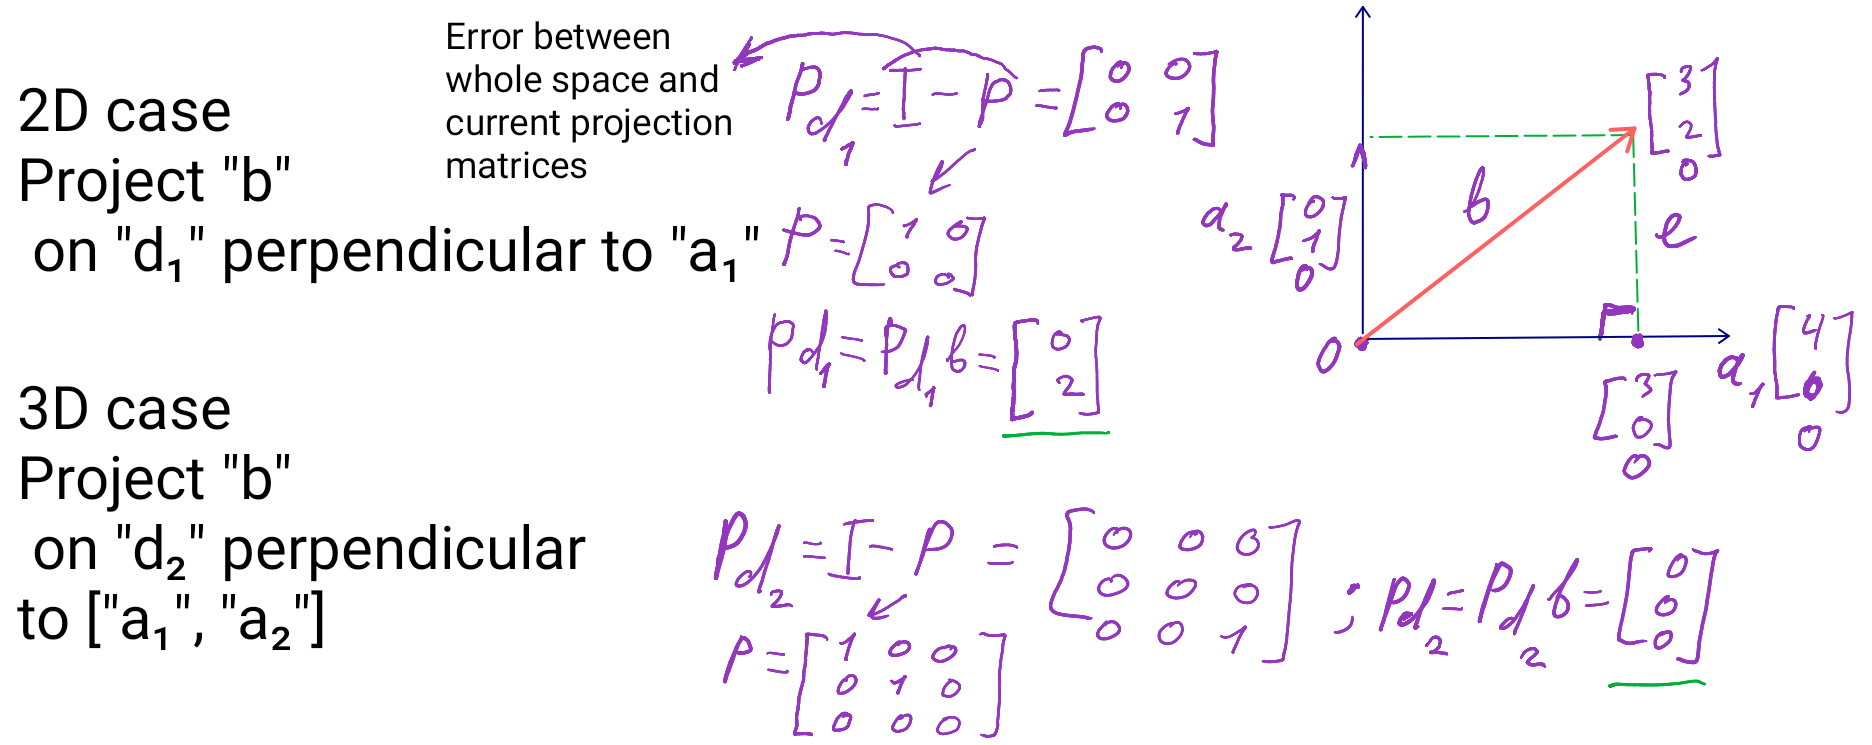
\includegraphics[height=6cm,width=1\textwidth,keepaspectratio]{AGLA2_for_slides_4.png}
        % \caption{caption_name}
        \label{fig:AGLA2_for_slides_4.png}
    \end{figure}
\end{frame}

\begin{frame}[t]{Projection}
    \framesubtitle{Case study: Reinforcement Learning fitness function}
    \vspace{-0.75cm}
    \begin{columns}[T,onlytextwidth]
        \begin{column}{0.49\textwidth}
            \begin{block}{Goal}
                It is necessary for the robot to move in a straight line in all directions, as well as as as efficiently as possible. 
                
                The efficiency criteria are: course deviation error, max velocity and clearance.
            \end{block}
            \vspace{-0.5cm}
            \begin{flalign*}
                F = \omega_1X_z + \omega_2\frac{1}{|err| + \varepsilon}+ \omega_3(P_{d_{real}}\vec{X})\text{, where} \\
                err = |(I-P_{d_{real}})(I-P_{n_{pl}})\vec{X}|,\\
                \text{$P_{*}$ -- projection matrix, $\omega_{*}$ -- weight coeffs.}
            \end{flalign*}
        \end{column}
        \begin{column}{0.49\textwidth}
            \begin{figure}[H]
                \centering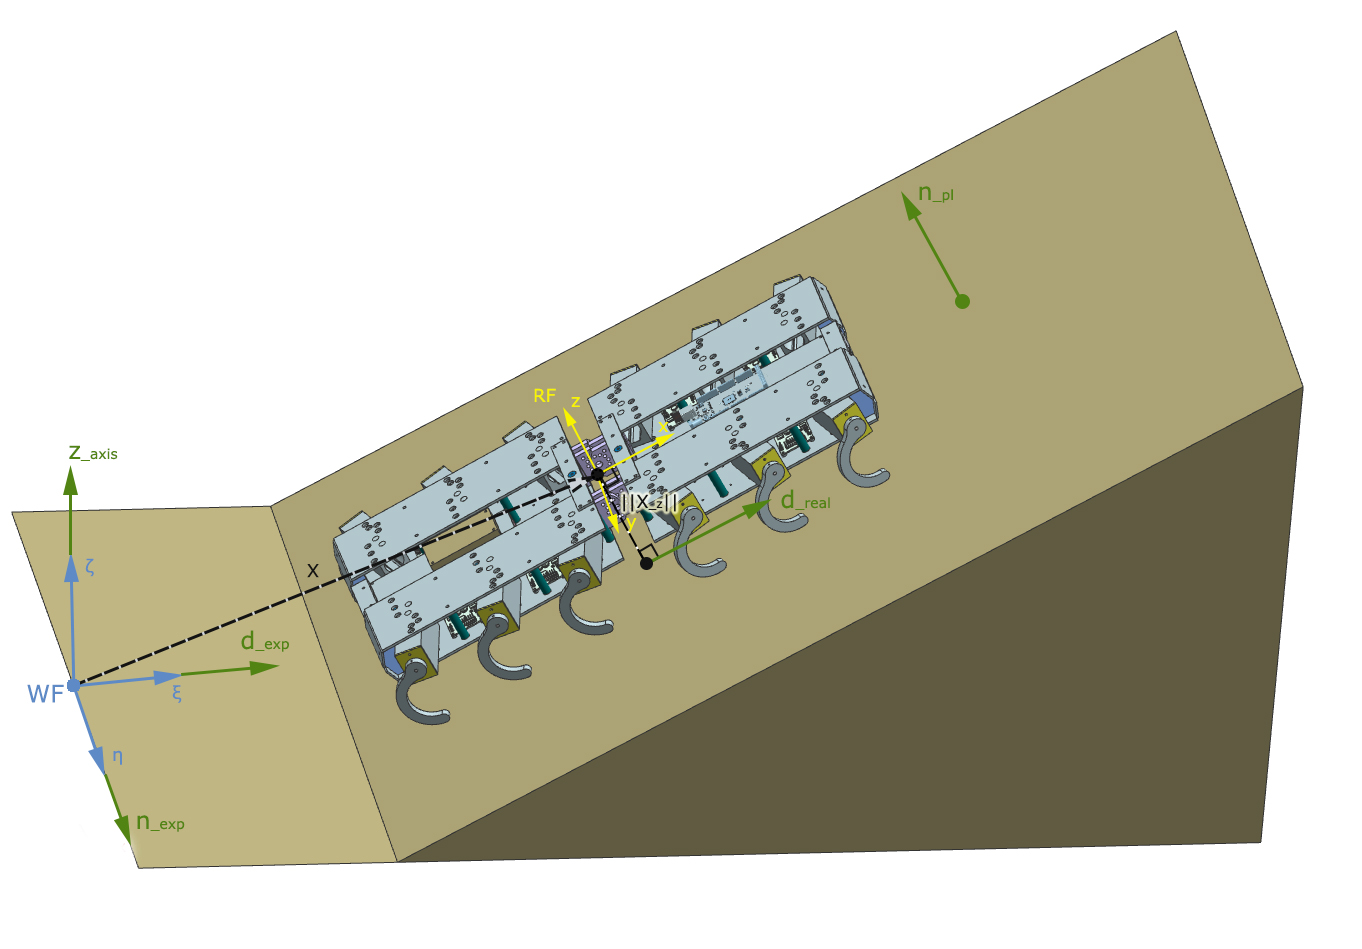
\includegraphics[height=6cm,width=1\textwidth,keepaspectratio]{strirus_full_body_on_plane_first.jpg}
                \caption*{\large StriRus -- task description}
                \label{fig:strirus_full_body_on_plane_first.jpg}
            \end{figure}
        \end{column}
    \end{columns}

\end{frame}


\begin{frame}[t]{Test 1, Solutions}
    \framesubtitle{Task 3}
    \begin{enumerate}
        \item Find the matrix product $AB$ if $A=\begin{bmatrix}x & -2 & -1 \\ 4 & 1 & -4 \end{bmatrix}$, $B=\begin{bmatrix} -5 & 1 \\ 1 & -3 \\ 2 & x \end{bmatrix}$
        \item Find the largest possible value of determinant $(AB)$.
    \end{enumerate}
    \end{frame}

\begin{frame}[t]{Test 1, Solutions}
\framesubtitle{Task 4}
(3 points)  Point $A$ has coordinates (5; -1; 8) in the old coordinate system. Find its coordinates in the new coordinate system obtained from the initial one by transferring the origin to point $N$ that has coordinates (33; -1; 2) in the old coordinate system.
\end{frame}

\begin{frame}[t]{Test 1, Solutions}
    \framesubtitle{Task 5}
    (3 points) Subspace $S$ of $\mathbb{R}^3$ is formed by linear combination of vectors $v_1$ and $v_2$. Find a vector $v$ that is orthogonal to $S$, if $v_1 = \begin{bmatrix}1 \\ 2\\ 3\end{bmatrix}$, $v_2 = \begin{bmatrix}4 \\ 5\\ 6\end{bmatrix}$
\end{frame}

\note{Обсудить когда будут линейно зависимые и линейно независимые результаты}

\begin{frame}[t]{Test 1, Solutions}
    \framesubtitle{Task 6}
    (3 points) Let \begin{equation}
        \mathbf{A}=\begin{bmatrix}
           0  & 1 & 0 \\
           0  & 0 & 1 \\
           1  & 0 & 0 
        \end{bmatrix}
        \end{equation}
    Find All \textbf{Natural} numbers ($k\in \mathbb{N}$) where: $A^k=A^{-1}$ ( Also you need to check if $A$ is invertible), Note that $A^k=\underbrace{A.A \dots A}_{k \ times} $
\end{frame}



\begin{frame}[t]{Reference material}
    % \framesubtitle{OnlineMschool}
    \Large
    \begin{itemize}
        \item \href{https://onlinemschool.com/math/library/matrix/rank/}{Matrix Rank (OnlineMschool)}
    \end{itemize}
\end{frame}

\fbckg{fibeamer/figs/last_page.png}
\frame[plain]{}

\end{document}